\documentclass{article}

\usepackage{graphicx}
\usepackage{wrapfig}
\usepackage{array}
\usepackage{hyperref}
\usepackage[left=2cm, right=2cm, top=2cm, bottom=3cm]{geometry}

\hbadness=10001
\hfuzz=100pt
\vfuzz=100pt

\title{Sozialwissenschaften}
\date{Q2 2022/2023}
\author{Paul SK \& Luca R}

\begin{document}
	\pagenumbering{gobble}
	\maketitle
	\newpage

	\pagenumbering{arabic}

	\section{Operatoren}
	Eine Übersicht der Operatoren kann \href{https://www.standardsicherung.schulministerium.nrw.de/cms/zentralabitur-gost/faecher/getfile.php?file=3947}{\underline{hier}} gefunden werden. 

	\section{Globale Strukturen und Prozesse}

	\subsection{Globalisierung}
	Globalisierung bezieht sich auf die zunehmende Vernetzung und Integration von Märkten, Kulturen und Gesellschaften auf der ganzen Welt, die durch die Liberalisierung des Handels, die technologischen Fortschritte und die Erleichterung des Personen- und Kapitalverkehrs ermöglicht wird.

	\subsubsection{Ursachen}
	Es gibt vier Hypothesen für die Ursache der Globalisierung:

	\begin{itemize}
		\item Ein kapitalistischer Weltmarkt begünstigt die Globalisierung, insbesondere die Arbeitsteilung und Spezialisierung
		\item Die Einführung digitaler Kommunikation und die Fortschritte in der Logistik ermöglichten Globalisierung
		\item Durch die USA wurden nach dem zweiten Weltkrieg Grundlagen für die wirtschaftliche und politishce Liberalisierung gelegt, die den Ausgangspunkt der Globalisierung bilden.
		\item Thatcher und Reagan setzten die Interessen der globalen Funktionselite durch und ermöglichten eine die Globalisierung begünstigende Deregulierung der Wirtschaft
	\end{itemize}

	Vermutlich ist nicht genau eine dieser Theorien richtig, vielmehr verstärkten sich die verschiedenen Gründe der Denationalisierung gegenseitig. Der Fortschritt in der Kommunikationstechnologie wird aber auf jeden Fall ein wichtiger Katalysator gewesen sein.

	\subsubsection{Dimensionen der Globalisierung}
	Die Globalisierung ist in vielen Bereichen des alltäglichen Lebens von Bedetung. Sie kann in 5 Dimensionen unterteilt werden.

	\paragraph{Wirtschaftliche Globalisierung}
	bezieht sich auf den Austausch von Waren, Dienstleistungen und Finanzmitteln auf globaler Ebene.	

	\paragraph{Politische Globalisierung}
	bezieht sich auf die Interaktion von Regierungen und politischen Institutionen auf globaler Ebene. Diese Dimension ist besonders erkennbar anhand von Institutionen wie der EU, der UN, den G7 und den G20. Handelsabkommen sind ebenfalls ein Merkmal dieser Entwicklung.

	\paragraph{Kulturelle Globalisierung}
	bezieht sich auf den Austausch von Kulturgütern, wie z.B. Musik, Filmen und Literatur, aber auch Riten und Religionen auf globaler Ebene. Die kulturelle Globalisierung hat drei Grundursachen:

	\begin{enumerate}
		\item Durch die ökonomische Globalisierung is eine Weltgesellschaft entstanden, in der Kapital und Waren über die ganze Erde bewegt und die Menschen immer mobiler werden
		\item Weltweite Migrationsprozesse tragen zu einer Vermischung der unterschiedlichsten Kulturen bei
		\item Die Entwicklung von Massenmedien wie Fernsehen, Radio und Internet bilden die Basis für die weltweite Vernetzung von Kulturen und Künsten
	\end{enumerate}

	Bei Debatten über die kulturelle Globalisierung ist die Frage häufig, ob diese Form der Globalisierung eher Vielfalt oder Nivellierung bringt. Einerseits finden die Begegnungen zweier Kulturen häufig nicht gleichberechtigt statt, was die Gefahr einer wirtschaftlichen und kulturellen Dominanz der Industriestaaten und einer weltweiten Standadisierung birgt. Andererseits könnte diese Entwicklung auch der Weg zu einer globalen demokratischen Zivilgesellschaft sein, die allerdings noch eine globale Identität finden muss. Somit kann die soziokulturelle Globalisierung sowohl Vielfalt als auch die Unterdrückung anderer Perspektiven und Einflüsse bringen.

	\paragraph{Globalisierung der Umweltprobleme}
	bezieht sich auf die Auswirkungen von Aktivitäten auf globaler Ebene auf die Umwelt, wie z.B. den Klimawandel und die Zerstörung von Ökosystemen. Diese globalen Probleme müssen auch global gelöst werden, da sie von einer Vielzahl an Akteuren verursacht und einen großen Einfluss auf viele Menschen haben, deren Lebensgrundlage teilweise drastisch zunichte gemacht wird.

	\paragraph{Globalisierung der Arbeitsmärkte}
	bezieht sich auf die zunehmende Verflechtung und Deregulierung von Arbeitsmärkten auf globaler Ebene. Ein wichtiges Merkmal dieser Entwicklung ist die Auslagerung der Produktion (\textit{Offshoring}) aus den Industrieländern in Entwicklungsländer, da die Lohnkosten in diesen Staaten vergleichsweise niedrig sind. Ein weiterer Vorteil sind die niedrigen Sozialabgaben. Arbeitnehmer in den Entwicklungsländern müssen dafür erhebliche Risiken, beispielsweise im Falle einer Arbeitsunfähigkeit, auf sich nehmen. Dennoch sind die Stellen bei Großkonzernen angesichts der hohen Arbeitslosenrate in den Entwicklungsländern beliebt. Auch schreitet durch die Ausbreitung der "Global Player" die Industrialisierung voran. Auch steigt der Bildungsstandard der Bevölkerung in den Entwicklungsländern, da mehr qualifizierte Arbeitskräfte benötigt werden. Dennoch bleiben auch diese Arbeiter unterbezahlt. Auch die Arbeitsbedingungen sind mit den Standards der Industrieländer nicht zu vergleichen.

	\subsubsection{Globalisierungskritik}
	Obwohl die Globalisierung auf den ersten Blick viele Vorteile bringt, gibt es einige Menschen, die diese Entwicklung durchaus kritisch sehen. Argumente dieser Menschen sind:

	\begin{itemize}
		\item Größere Kluft zwischen Arm und Reich: Reichtum konzentriert sich auf immer weniger Menschen
		\item Großer Unterschied zwischen den Industrieländern und den Ländern des globalen Südens
		\item Globalisierungspolitik bezieht sich häufig auf liberalisierte Märkte und die Interessen der Großkonzerne, selten jedoch auf Menschenrechte oder ökologische Probleme
		\item Es herrschen zu hohe Ansprüche an das Wirtschaftswachstum
		\item Finanzkrisen, die von den Wohlhabenden verursacht wurden, werden auf die Allgemeinheit abgewälzt
	\end{itemize}

	\subsubsection{Global Governance}
	Global Governance ist ein Aspekt der politischen Dimension der Globalisierung: aufgrund von wachsenden globalen Problemen und einer stetig steigenden Vernetzung gibt es einen Bedarf an einer Form des globalen Regierens. Governance ist dabei sowohl der Inhalt als auch der Prozess des Regierens. Momentan ist dieser Bereich hauptsächlich ein Flickenteppich aus begrenzt zuständigen internationalen Institution (z.B. die WTO oder die WHO). Mechanismen oder Strukturen zur Koordination gibt es kaum. Ausnahmen sind die exklusiven G7- und G20-Gipfeltreffen. Es fehlen problemfeldübergreifende Instanzen und einheitliche Verhältnisse zwischen internationalen und nationalen Regeln.

	\paragraph{G7 / G8}
	Die G8 waren ursprünglich eine Gruppe der 8 größten Industrienationen. Ihre gehörten Deutschland, Frankreich, Großbritannien, Italien, Japan, Kanada, die USA und Russland sowie die EU als Beobachter an. Seit der Annektion der Krim 2014 wird Russland aus der Gruppe ausgeschlossen, weshalb man nunmehr von den G7 spricht. Die Regierungschefs dieser Gruppe trifft sich jährlich auf einem Gipfeltreffen. Der Vorsitz wechselt jährlich, für 2023 hat Japan den Vorsitz inne.
	Auch, wenn die G7 ursprünglich die größten Industrienationen repräsentieren sollten, hat sich die Weltwirtschaft in den letzten 50 Jahren stark verändert, wehalb diese Gruppe heutzutage mehr eine westliche Wertegemeinschaft ist.

	\paragraph{G20}
	Die G20 sind ähnlich zu den G7 ein informelles Forum, welches ca. 2/3 der Weltbevölkerung und mehr als 80\% des globalen BIP abdeckt. Neben den Staaten der G7 und der EU gehören unter anderem auch Russland, China, Saudi Arabien und Indien zu diesem Format- es soll die 20 größten Industrie- und Schewllenländer repräsentieren. Die Gipfeltreffen unter der wechselnden Elietung eines der Mitgliedsstaaten führt in der Regel zu einer gemeinsamen Abschlusserklärung, die allerdings völkerrechtlicht nicht bindend ist. Kritiker bemängeln an den G20, dass sie eine unrepräsentative Gruppe darstellen, undurchsichtige und undemokratische Entscheidungen treffen, und dass ihre Beschlüsse oft nur Absichtserklärungen bleiben. Zudem konzentrieren sich die G20 hauptsächlich auf wirtschaftliche Themen und vernachlässigen andere globale Herausforderungen, die beispielsweise humnatärer oder ökologischer Natur sind.


	\subsection{Internationale Beziehungen}

	\subsubsection{Politische Handlungsstrategien}

	\paragraph{Hegemoniale Ordnung}
	Ein einzelner mächtiger Staat bindet andere Staaten über Abhängigkeiten an sich und sorgt auf diese Weise für Stabilität und Frieden. Außerdem profitieren die abhängigen Staaten von den durch die Hegemonialmacht bereitgestellten Wirtschaftsbeziehungen.

	\paragraph{Imperialistische Ordnung}
	Ein einzelner Staat erobert und kontrolliert große Teile der Welt und macht die besetzten Gebiete durch verschiedene Methoden von sich abhängig.

	\paragraph{Unilateralismus}
	Jeder Staat sorgt unabhängig von anderen Staaten für die Durchsetzung der eigenen Interessen, notfalls auch gegen die Wünsche anderer Staaten.Zur Erfüllung der eigenen Interessen sind auch Gewalt und Kriege valide Mittel.

	\paragraph{Multilateralismus}
	Verschiedene Staaten agieren gemeinsam anhand von allgemeinen Regeln und Prinzipien. Dabei versuchen diese Staaten, gemeinsame Interessen durchzusetzen. Wichtig ist, dass die gemeinsamen Prinzipien auch bei gegensätzlichen Interessen nicht verletzt werden und Konflikte nicht mit Gewalt, sondern durch Diplomatie und Kompromisse gelöst werden.

	\subsubsection{Freihandel und Protektionismus}
	\paragraph{Freihandel}
	Freihandel beschreibt den Handel von Waren und Dienstleistungen zwischen Ländern ohne oder mit nur sehr wenigen Handelshemmnissen wie beispielsweise Zöllen, Quoten oder anderen Beschränkungen. Die Idee des Freihandels hat eine lange Geschichte, die bis ins 18. Jahrhundert zurückreicht. Im Laufe der Geschichte wurden zahlreiche Freihandelsabkommen geschlossen (bspw. das General Agreement on Tariffs and Trade \textit{GATT} oder die \textit{WTO}), um den internationalen Handel zu erleichtern und zu fördern. Allerdings gibt es auch Kritik am Freihandel, da er zu einer ungleichen Verteilung von Wohlstand und Macht zwischen den Ländern führen kann und insbesondere in Entwicklungs- und Schwellenländern negative Auswirkungen auf die lokale Wirtschaft und Gesellschaft haben kann.

	\paragraph{Protektionismus}
	Protektionismus beschreibt das Bemühen eines Staates, seine eigene Wirtschaft zu schützen, indem er Handelsbeschränkungen und Zölle auf importierte Waren und Dienstleistungen einführt. Der Protektionismus kann auch in Form von Subventionen für heimische Produzenten oder der Einführung von Handelshemmnissen wie beispielsweise Einfuhrquoten auftreten. Protektionistische Maßnahmen haben oft zum Ziel, einheimische Arbeitsplätze zu schützen und den Wohlstand im eigenen Land zu sichern. Ein bekanntes Beispiel ist die gemeinsame Agrarpolitik der Europäischen Union, die den heimischen Bauern Subventionen gewährt, um ihre Produkte wettbewerbsfähiger zu machen.


	\subsection{Internationale Friedenspolitik}

	\subsubsection{Alte und neue Kriegsursachen}
	Seit dem zweiten Weltkrieg hat sich der Kriegsbegriff und insbesondere auch die Kriegsursachen stark verändert.

	\paragraph{Alte Kriegsursachen}
	Früher waren Kriege vor allem in Territorialansprüchen, der Herrschaftssicherung und in anderen Herrschaftsinteressen begründet. Dazu gehört auch die Machtkonkurrenz verschiedener Herrscher in einer Region. Außerdem wurden Kriege genutzt, um von innerstaatlichen Problemen abzulenken oder Rohstoffe zu sichern. Darüber hinaus führten auch Fehleinschätzungen bezüglich der Stärke und den Absichten anderer Staaten zu Kriegen. Klassische Kriege sind außerdem stark davon geprägt, dass es sich zumeist um Konflikte zwischen zwei oder mehr Staaten handelte.

	\paragraph{Neue Kriegsursachen}
	Heutzutage gibt es vermehrt innerstaatliche Konflikte, die durch soziale bzw. ökologische Probleme wie Armut, Überbevölkerung, starke soziale Ungerechtigkeit oder Umweltzerstörung verursacht werden. Häufig entstehen Konflikte auch durch ethnische oder kulturelle Unterschiede zwischen Bevölkerungsgruppen innerhalb eines Staates. Diese Unterschiede liegen auch häufig an der willkürlichen Grenzziehung durch Kolonialmächte. Diese ethnischen Konflikte werden teilweise auch durch die Unterdrückung bestimmter Gruppen durch die Regierung eines Staates begünstigt. Außerdem gewinnt der Terrorismus, der zumeist religiös oder national begründet ist, zunehmend an Bedeutung in weltweiten Konflikten.

	\subsubsection{Definitionen von Konflikten}
	Die \textit{Arbeitsstelle Kriegsursachenforschung} (\textit{AKUF}) in Hamburg unterscheidet zwischen 5 Arten von Konflikten:

	\paragraph{Antiregime-Kriege}
	sind Kriege, in denen um innerstaatliche Themen wie den Sturz einer Regierung, der Veränderung eines politischen Systems bzw. einer Gesellschaftsordnung oder den Erhalt der beiden letzteren gekämpft wird. Der Bürgerkrieg in Syrien war beispielsweise ursprünglich ein Antiregimekrieg

	\paragraph{Autonomie- und Sezessionskriege}
	haben die Lösung einer Region oder die Sezession eines Staates aus einem Staatenbund zum Ziel. Ein Beispiel für Autonomiekriege sind die Tschetschenienkriege, in denen die Kaukasusrepublik Tschetschenien versuchte, sich unabhängig von Russland zu erklären.

	\paragraph{Zwischenstaatliche Kriege}
	sind Kriege im klassischen Sinne zwischen zwei Staaten mit etablierten Regierungen und Territorien. Der Ukrainekrieg ist ein aktuelles Beispiel für so einen Konflikt.

	\paragraph{Dekolonialisierungskriege}
	bezeichnen Kriege, in denen um die Befreiung von Kolonialherrschaft gekämpft wird. Mit dem Rückgang an Kolonien ist diese Kriegsform immer seltener geworden; ein bekanntes Beispiel ist der Falklandkrieg zwischen Argentinien und dem Vereinigten Königreich um die Falklandinseln.

	\paragraph{Sonstige Kriege}
	fassen alle übrigen Kriegsformen oder Mischformen der verschiedenen Konfliktformen zusammen.

	\subsubsection{Philosophische Meinungen zum Frieden}

	\paragraph{Immanuel Kant}
	Der deutsche Philosoph Kant legt in seiner Schrift "Zum ewigen Frieden" drei Artikel fest, die einen dauerhaften Friedenszustand gewähren sollen. Der erste Artikel besagt, dass jeder Staat eine demokratische (wörtlich "republikanische") Verfassung haben sollte, da nur diese die Gleicheit der Bürger und die Abhängigkeit von einer einzigen gemeinsamen Gesetzgebung garantiert.
	Der zweite Artikel besagt, dass die einzelnen Staaten sich ohne Aufgabe ihrer staatlichen Souveränität zu einem "Friedensbund" zusammenschließen sollen, da Friedensverträge nach einem Krieg meist nur von kurzer Dauer sind. Ein dauerhafter Friedensbund hingegen soll eine Gemeinschaft zum Erhalt von Fireden und Freheit sein.
	Im dritten Artikel beschreibt Kant, dass ein Fremder auf dem Territorium eines anderen Volkes ein Gast- bzw. Besuchsrecht genießen muss, sodass ihm nicht feindlich gegenüber gestanden wird.

	\paragraph{Thomas Hobbes}
	Hobbes sagt, dass der einzige Weg, wie die Menschen einen von ihm skizzierten "andauernden Kriegszustand" verlassen können, ist, dass sie ihre gesamte Macht und ihren Willen auf eine andere Person oder eine Personengruppe übertragen. Dafür muss nach Hobbes "jeder einen Vertrag mit jedem schließen", der besagt, dass der eigene Wille auf die vorher beschriebene Person oder Gruppe übergeht. Diese Institution, unter der der Wille aller vereinigt wird, nennt er "Leviathan", der allen Frieden und Schutz bringt. Nur auf diesem Weg sei es möglich, dass die Menschen sich nicht länger untereinander bekriegen.
 
	\subsection{Vereinte Nationen}
	Die Vereinten Nationen (UN) sind eine internationale Organisation, die 1945 gegründet wurde, um zwischenstaatliche Zusammenarbeit und Koordination in verschiedenen Bereichen wie Frieden und Sicherheit, Wirtschaft und Entwicklung, Umwelt und Menschenrechte zu fördern. Die UN besteht aus 193 Mitgliedsstaaten und hat ihren Hauptsitz in New York City.

	\subsubsection{Entstehung \& Geschichte}
	\begin{itemize}
		\item \textbf{1939} Scheitern des nach dem ersten Weltkriegs etablierten Völkerbundes mit Ausbruch des Zweiten Weltkriegs
		\item \textbf{1941} Erarbeitung der \textit{Atlantik-Charta} durch Churchill und Roosevelt
		\item \textbf{1942} Deklaration der Vereinten Nationen durch 26 Staaten mit Berufung auf die Atlantik-Charta
		\item \textbf{1943} \textit{Moskauer Deklaration} der vier Großmächte USA, Großbritannien, China und der Sowjetunion mit dem  Ziel der Schaffung einer internationalen Organisation zur Aufrechterhaltung des Friedens
		\item \textbf{1945} Fertigstellung der \textit{Charta der Vereinten Nationen} und Unterzeichnung durch 51 Staaten
		\item \textbf{1956} Etablierung einer Trennung von "Friedenssicherung" und "Friedensschaffung" zur Emöglichung einer Konsensfindung im Sicherheitsrat
		\item \textbf{1971} Die Volksrepublik China wird als einziger Vertreter des chinesischen Volkes anerkannt; sie erhält auch den Sitz Chinas im Sicherheitsrat. Taiwan (Republik China) ist seitdem nicht mehr in der UNO vertreten
		\item \textbf{1972} Die BRD und die DDR werden beide in die UN aufgenommen
		\item \textbf{1992} Übernahme des UN-Mandats der Sowjetunion durch die Russische Föderation
		\item \textbf{1994} Versagen der UN-Blauhemsoldaten im Völkermord in Ruanda
		\item \textbf{1995} Geiselnahme von UN-Soldaten im Jugoslawienkrieg
		\item \textbf{2000} Nach dem Versagen der UN-Friedenstruppen in Ruanda, Jugoslawien und Somalia wird eine Überarbeitung des Friedenssicherungskonzeptes der UN gefordert
	\end{itemize}

	Die UN haben heute 193 Mitglieder.

	\subsubsection{Organe}

	\paragraph{Die Generalversammlung}
	ist die Vollversammlung aller UN-Mitgliedsstaaten. Jeder Mitgliedsstaat kann bis zu fünf Abgeordnete zu den Treffen entsenden. Die Versamlung empfiehlt völkerrechtlich nicht bindende Resokutionen ud beschließt den UN-Haushalt und darf sich mit praktisch jeder Frage von internationaler Bedeutung befassen, solange sie nicht gleichzeitig vom UN-Sicherheitsrat behandelt wird. Die UN-Vollversammlung ist kein Weltparlament und nicht hinreichend legitimiert, da die Teilnehmer nur indirekt demokratisch (in Staaten mit demokratischem System) oder gar nicht (in nicht-demokratischen Staaten) legitimiert sind.


	\subparagraph{Abstimmung}
	Jeder Staat verfügt über eine Stimme, unabhängig von seiner Wirtschaftskraft oder Bevölkerugnszahl. In der Regel wird mit einfacher Mehrheit entschieden, es werden nur Ja-Nein-Stimmen in das Ergebnis mit einbezogen. In bestimmten Fragen wird mit einer Zwei-Drittel-Mehrheit entschieden:

	\begin{itemize}
		\item Fragen bezüglich des Weltfriedens und der internationalen Sicherheit
		\item Die Wahl der nicht-ständigen Mitglieder des Sicherheitsrates
		\item Die Aufnahme neuer Mitglieder
		\item Der Ausschluss eines Staates aus den UN
		\item Budgetfragen
	\end{itemize}

	\subparagraph{Sitz}
	New York City

	\paragraph{Der Sicherheitsrat}
	Der Sicherheitsrat ist ein Gremium aus 15 Mitgliedern, von denen 5 (Frankreich, Russland, USA, China, Großbritannien) einen ständigen Sitz 10 weitere einen nicht-ständigen Sitz haben (derzeit Albanien, Brasilien, Gabun, Ghana, Vereinigte Arabische Emirate, Ecuador, Japan, Malta, Mosambik, Schweiz). Der Sicherheitsrat hat die primäre Aufgabe, den Weltfrieden und die internationale Sicherheit zu gewährleisten. Er ist befugt, verbindliche Entscheidungen zu treffen. Die Entscheidungen des Sicherheitsrates unterliegen keiner wirksamen Rechtskontrolle. 

	\subparagraph{Mitgliederauswahl}
	Die nicht-ständigen Sitze des Sicherheitsrates  werden nach regionalen Gruppen ausgesucht und dann von der UN-Vollversammlung bestätigt:

	\begin{itemize}
		\item Drei afrikanische Länder
		\item Zwei asiatische Länder
		\item Zwei lateinamerikanische Länder
		\item Ein osteuropäisches Land
		\item Zwei aus Westeuropa, Kanada, Australien oder Neuseeland
	\end{itemize}

	\subparagraph{Abstimmung}
	Ein Beschluss des Sicherheitsrates benötigt die Stimmen von neun Mitgliedern. Allerdings müssen auch die fünf ständigen Mitglieder für einen Beschluss immer zustimmen, wodurch diese ein \textit{Vetorecht} haben. Eine Ausnahme sind Verfahrensfragen, bei denen die ständigen Mitglieder kein Veto haben. Das Nichterscheinen zu Sitzungen kann je nach Auslegung als Stimmenthaltung oder als fehlende Zustimmung betrachtet werden. Diese Kontroverse ist insbesondere im Hinblick auf die Blockierung des Sicherheitsrates im Zuge der "Politik des leeren Stuhls" der UdSSR in Folge der Verweigerung des ständigen Sicherheitsratsmandats gegenüber der neuen chinesischen Regierung durch die Westmächte und der Auslegung dieser als Enthaltung durch die westlichen Staaten problematisch.

	\subparagraph{Sitz}
	New York City

	\subparagraph{Kritik}
	Durch das Vetorecht wird der Sicherheitsrat häufig blockiert und ist daher in vielen Fällen nicht beschlussfähig ($\rightarrow$ \textit{Effizienz})

	\paragraph{Der internationale Gerichtshof}
	Der internationale Gerichtshof (nicht zu verwechseln mit dem internationalen \underline{Straf}gerichtshof) entscheidet Streitfragen zwischen zwei oder mehr Staaten. Wichtig ist, dass nur Staaten Parteien können, nicht jedoch andere Völkerrechtssubjekte. Außerdem müssen Staaten sich dem IGH explizit unterwerfen, er ist also nicht allgemein zuständig. Derzeit haben 73 Staaten (u.A. Deutschland) eine generelle Unterwerfungserklärung an den IGH abgegeben. Er entscheidet anhand von internationalen Abkommen, dem internationalen Gewohnheitsrecht und den von zivilisierten Staaten anerkannten allgemeinen Rechtsgrundsätzen. Das Gericht besteht aus 15 Richtern, die alle unterschiedlichen Staaten angehören müssen und für neun Jahre von der Generalversammlung und dem Sicherheitsrat gewählt werden.

	\subparagraph{Sitz}
	Den Haag (Niederlande)

	\paragraph{Das Sekretariat}
	Das UN-Sekretariat ist ein Verwaltungsorgan der UN. Unter anderem oraganisiert es Konferenzen, verfasst Studien und Berichte und stellt einen Haushaltsplan auf. Der UN-Genealdekretät (momentan: António Guterres) ist der wichtigste Repräsentant der UN.

	\subparagraph{Sitz}
	\begin{itemize}
		\item New York City (Hauptsitz)
		\item Genf, Nairobi, Wien (Außenstellen)
	\end{itemize}

	\paragraph{Der Wirtschafts- und Sozialrat}
	Dieser Rat ist ein weiteres Organisationsorgan und koordiniert außerdem 17 weitere Sonderorganisationen. Seine Aufgaben sind:

	\begin{itemize}
		\item Die Hebung des allgemeinen Lebensstandards
		\item Die Formulierung von Lösungsvorschlägen für internationale wirtschaftliche, soziale und gesundheitliche Probleme
		\item Die Förderung der internationalen Kooperation in Kultur und Erziehung
		\item Die Förderung der Menschenrechte
	\end{itemize}

	Er hat 54 Mitglieder, unter denen die Entwicklungsländer überpropotional stark vertreten sind. Der Ratspräsident wird jedes Jahr mit einer einfachen Mehrheit gewählt (momentan: Collen Vixen Kelapile). 

	\subparagraph{Sitz}
	New York City

	\paragraph{Der Treuhandrat}
	Dieses Gremium war mit der Verwaltung von ehemaligen Kolonien beauftragt (sogenannte Treuhandgebiete). Seit der Entlassung des letzten Treuhandgebietes 1994 ist er inaktiv. Er hat daerzeit keine Aufgaben

	\subparagraph{Sitz}
	New York City

	\paragraph{Verschiedene Sonderorganisationen}
	Weitere Organisationen der UN sind unter anderem die Welthandelsorganisation (WTO) und die Weltgesundheitsorganisation (WHO).

	\subsubsection{UN-Friedenssicherungspolitik}
	Die Friedenssicherungspolitik der UN besteht momentan haupptsächlich aus Beobachtungsmissionen und Friedenssicherungsmission, in denen die sogenannten "Blauhemsoldaten" eingesetzt werden. Diese stammen häufig eher aus Ländern des globalen Südens, da die Industriestaaten Verluste unter ihren Truppen meist vermeiden wollen, unter anderem auch aus Wahlkampfgründen. Für ärmere Länder stellen diese Einsätze hingegen einen Prestigegewinn und eine Einnahmequelle dar.

	\paragraph{Grundsätze}

	\subparagraph{Konsens der Teilnehmer}
	\begin{itemize}
		\item Legitimierugn des Einsatzes
		\item UN-Truppen werden keine Konfliktpartei
		\item Beendigung des Friedenseinsatzes jederzeit möglich
	\end{itemize}
	
	\subparagraph{Unparteilichkeit}
	\begin{itemize}
		\item unparteiischer Umgang mit den Konfliktparteien
		\item beeinflusst nicht die Ausführung des Mandats
	\end{itemize}

	\subparagraph{Nicht-Anwendung von Gewalt}
	Ausnahmen nur bei
	
	\begin{itemize}
		\item Selbstverteidigung
		\item Verteidigung des Mandats
		\item "Robuste" Friedensmissionen
	\end{itemize}

	Ein Einsatz von Gewalt muss genau abgewogen werden und stets das letzte Mittel sein.

	\paragraph{Konzept der Schutzverantwortung}
	\subparagraph{System aus}
	
	\begin{enumerate}
		\item Nationalen Maßnahmen
		\item Frühwarnmechanismen
		\item Eingriff der Mitgliedsstaaten der UN
	\end{enumerate}

	\subparagraph{Verhinderung / Beendigung von}

	\begin{itemize}
		\item ehtnischen Säuberungen
		\item Verbrechen gegen die Menschlichkeit
		\item Kriegsverbrechen
		\item Völkermorden
	\end{itemize}

	\subsection{Die NATO}
	Die \textit{North Atlantic Treaty Organization} ist ein Verteidigungsbündnis aus 31 europäischen und amerikanischen Staaten. Gleichzeitig versteht die NATO sich auch als Wertegemeinschaft demokratischer Staaten. Ursprünglich diente das Bündnis den USA für ihre Politik im \textit{Kalten Krieg} gegen die Sowjetunion. Sie ist eines der wichtigsten Verteidigungsbündnisse weltweit.

	\subsubsection{Entstehung \& Entwicklung}
	Aus Sorge vor einer sowjetischen Ausbreitung und einer etwaigen Agression baten verschiedene europäische Staaten die USA als eine Art Schutzmacht um militärischen Beistand. Der Nordatlantikvertrag wurde dann 1949 von den BeNeLux-Staaten, Dänemark, Frankreich, dem Vereinigten Königreich, Island, Italien, Kanada, Norwegen, Portugal und den USA unterzeichnet. Das dem Bündnis zugrundeliegende Prinzip besagt, dass ein Angriff auf einen einzelnen NATO-Partner wie ein Angriff auf alle Teilnehmer behandelt werden solle. (West)Deutschland trat der NATO 1955 bei. Heute hat die NATO 28 Mitglieder. Seit ihrer Gründung hat sich die NATO stark verändert: statt reiner Selbstverteidigung erfüllte die NATO auch Aufgaben wie Krisenmanagement im euro-atlantischen Raum. Außerdem wurde nach dem 11. September 2001 erstmals der Verteidigungsfall durch die USA ausgerufen, sodass NATO-Truppen in Afghanistan einmarschiert sind.

	\newpage

	\subsubsection{Aufbau \& Organe}

	\begin{figure}[!ht]
		\centering
  		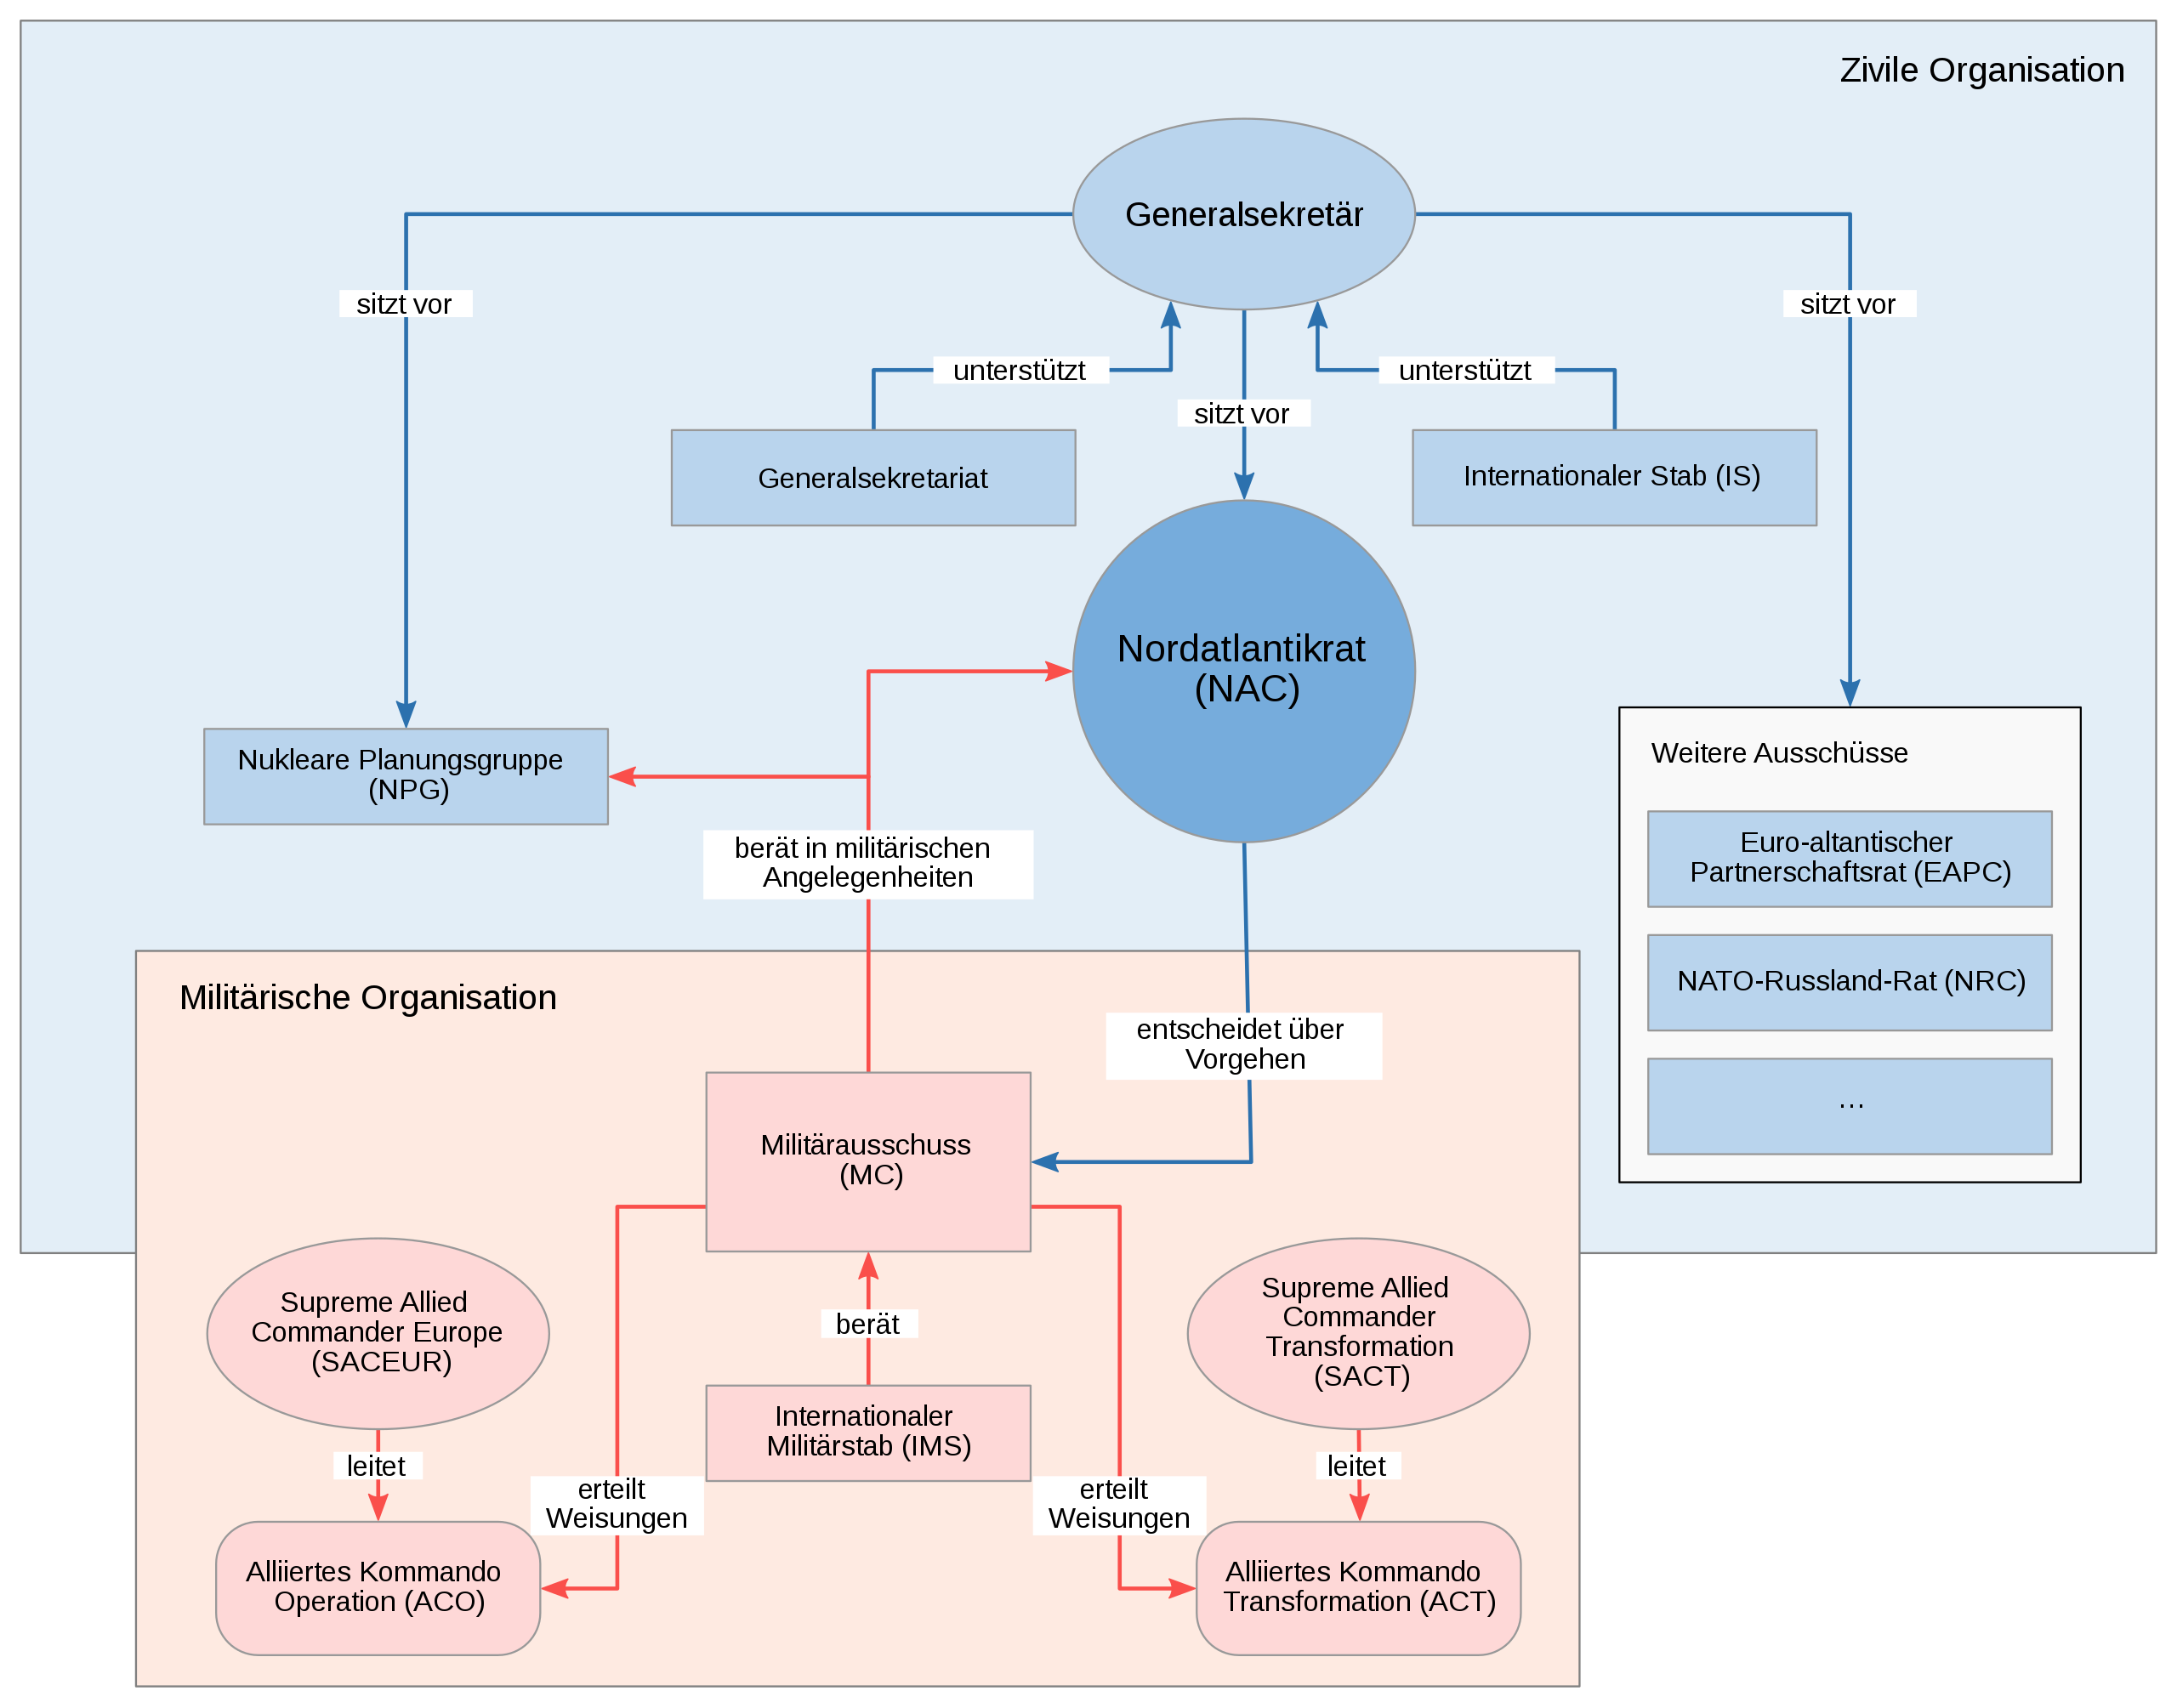
\includegraphics[width=45em]{nato_aufbau.png}
  		\caption{Der Aufbau der NATO}
  		\label{fig:nato_aufbau}
	\end{figure}

	\paragraph{Nordatlantikrat}
	Der Nordatlantikrat ist das höchste Entscheidungsgremium der NATO und kümmert sich um die politische Konsultation und Koordination.

	\paragraph{NATO-Generalsekretär}
	Der Generalsekretär (momentan: Jens Stoltenberg) ist Vorsitzender des Nordatlantikrats und der Hauptrepräsentant der NATO. Bisher war dies immer ein Europäer.

	\paragraph{Alliiertes Kommando Operationsführung}
	Diese Institution leitet die militärischen Einsätze der NATO. Den Oberbefehl hat den \textit{Supreme Allied Commander Europe}, der bisher immer ein Amerikaner war.

	\subsection{Bedeutung der Menschenrechte}

	\subsubsection{Geschichte}
	Im Laufe der Jahrhunderte wurden durch verschiedene Völker immer wieder neue Menschenrechte von den damaligen Herrschern erkämpft. Wichtige Meilensteine auf diesem Weg sind:

	\begin{itemize}
		\item \textbf{1776} "Declaration of Rights" im Tahmen der Amerikanischen Unabhängigkeit
		\item \textbf{1789} Erklärung der Menschen- und Bürgerrechte im Zuge der Französischen Revolution
		\item \textbf{1948} Allgemeine Erklärung der Menschenrechte durch die UN
		\item \textbf{1950} Europäische Menschenrechtskonvention
		\item \textbf{1976} Weltpakete über bürgerliche und politische Rechte und über soziale und kulturelle Rechte der UN
	\end{itemize}

	\subsubsection{Merkmale}
	Menschenrechte sind

	\begin{itemize}
		\item Angeboren und unveräußerlich
		\item Individuell; jeder Mensch ist ein Individuum
		\item Egalitär; d.h. für jeden gleichermaßen gültig
		\item Universell
		\item Unteilbar; die Menschenrechte sind alle miteinander verflochten
	\end{itemize}

	\subsubsection{Europäische Menschenrechtskonvention}
	Die EMRK ist ein 1953 in Kraft getretener Vertrag, der eine große Bandbreite an geschützten Grundrechten garantiert und über den Europäischen Gerichtshof für Menschnrechte ein Kontrollsystem für die Einhaltung der Konvention bereitstellt. Vor dem Gerichtshof können Staaten und Organisationen, aber auch Individuen gegen Verstöße der Konvention klagen. Die Urteile des Gerichtshof sind verpflichtend

	\section{Europäische Union}

	\subsection{Stationen des europäischen Einigungsprozesses}
	\subsubsection{Ideen über die Zukunft Europas}
	\paragraph{Daten}
	\begin{itemize}
		\item \textbf{1945} Ende des zweiten Weltkriegs
		\item \textbf{1946} Churchill präsentiert seine Idee von den "Vereinigten Staaten von Europa"
		\item \textbf{1949} Gründung des Europarates in London
		\item \textbf{1946-1950} Monnetplan zur Erhöhung französischer und Reduktion deutscher Stahlproduktion
	\end{itemize}

	\paragraph{Hintergrund}
	Nach dem zweiten Weltkrieg wollten die europäischen Nationen keinen Krieg mehr. Durch Churchills "Vereinigte Staaten von Europa" sollten einzelne Nationen weniger wichtig sein als die große gemeinsame Sache. Der Monnetplan, benannt nach dem Franzosen Jean Monnet, sollte der Nährboden für ein Bündnis zwischen Deutschland und Frankreich sein: Frankreich fühlte sich durch die Überlegenheit der deutschen Stahlproduktion, mit der die französische nicht konkurrieren konnte, berdroht. Deutschland wurde nach wie vor als Bedrohung für den europäischen Frieden gesehen, auch aufgrund der Einflüsse aus den USA und der Sowjetunion. Der Monnetplan zielte daher darauf ab, die französische Stahlproduktion auszubauen und gleichzeitig die deutsche Stahlproduktion zu deckeln. 

	\subsubsection{Gründung und Aufbau der EU}
	\paragraph{Daten}
	\begin{itemize}
		\item \textbf{1950} Schuman stellt seine Pläne für die \textit{Europäische Gemeinschaft für Kohle und Stahl} vor
		\item \textbf{1951} Deutschland, Frankreich, Italien und BeNeLux-Staaten gründen EGKS
		\item \textbf{1957} EGKS-Staaten gründen \textit{Europäische Wirtschaftsgemeinschaft} mit Zollunion und gemeinsamer Agrarpolitik und die \textit{Europäische Atomgemeinschaft}
		\item \textbf{1965} EGKS, EWG und EUATOM werden zur \textit{Europäischen Gemeinschaft} fusioniert
	\end{itemize}

	\paragraph{Hintergrund}
	Durch die Kontrolle der französisch-deutschen Stahlproduktion durch eine gemeinsame Behörde sollte die Grundlage für weitere Kriege vollständig eliminiert werden. Die EGKS legte den Grundstein für eine europäische Zusammenarbeit, die durch die Folgeverträge der EWG, EURATOM und die EG weiter verstärkt wurde. Die früheren Erzfeinde Deutschland und Frankreich arbeiteten nun zusammen, was weitere Kriege unmöglich machen und der EU die erste Grundlage geben sollte.

	\subsubsection{Nord- und Süderweiterung}
	\paragraph{Daten}
	\begin{itemize}
		\item \textbf{1966} Der Luxemburger Kompromiss macht Entscheidungen per Mehrheitsprinzip möglich
		\item \textbf{1971} Ministerrat beschließt das Ziel der Errichtung einer \textit{Wirtschafts- und Währungsunion}
		\item \textbf{1973} Beitritt von Großbritannien, Irland und Dänemark
		\item \textbf{1979} Erste Direktwahlen des \textit{Europäischen Parlaments}
		\item \textbf{1981/1986} Beitritt von Griechendland, Portugal und Spanien
	\end{itemize}

	\paragraph{Hintergrund}
	Obwohl das EP prinzipiell seit der Gründung der EGKS bestand, waren die Mitglieder erst einmal nur Abgeordnete nationaler Parlamente. 1979 wurden dann erstmals Direktwahlen durch die Bürger der EG abgehalten.

	\subsubsection{Politische und ökonomische Vertiefung}
	\paragraph{Daten}
	\begin{itemize}
		\item \textbf{1986} Fusionierung der Gründungsverträge zur \textit{Einheitlichen Europäischen Akte}
		\item \textbf{1992} Gründung der \textit{Europäischen Union}; Beginn der \textit{Gemeinsamen Außen- und Sicherheitspolitik} sowie der polizeilich-justiziellen Zusammenarbeit
		\item \textbf{1995} Schengen-Abkommen; Beitritt von Finnland, Schweden und Österreich
	\end{itemize}

	\paragraph{Hintergrund}
	Durch die Zusammenlegung der Verträge in der EEA sollte die Zusammenarbeit nochmals gestärkt werden. Der Einigungprozess innerhalb der EG sollte durch einen Ausbau des Europäischen RAtes, durch die Kompetenzerweiterung des EP und durch die Abschaffung des \textit{Einstimmigkeitsprinzips} im Ministerrat effizienter gestaltet werden.
	Durch die Gründung der EU im \textit{Vertrag von Maastricht} sollte der wirtschaftliche Fokus des Staatenbundes um einen politischen Aspekt erweitert werden. Die Union sollte fortan auf drei Säulen aufbauen:

	\begin{enumerate}
		\item Die \textit{Europäische Gemeinschaft}
		\item Die \textit{Gemeinsame Außen- und Sicherheitspolitik} zur Verfolgung internationaler Interessen und schnellerer Reaktion auf Krisen
		\item Die Zusammenarbeit der Justiz- und Innenminister bezüglich 
		\begin{itemize}
			\item Asylpolitik
			\item Grenzkontrollen
			\item Einwanderungspolitik
			\item Drogenbekämpfung
			\item internationale Kriminalität
			\item Terrorismusbekämpfung
		\end{itemize}
	\end{enumerate}

	Zudem wurde eine Wirtschafts- und Währungsunion beschlossen

	\subsubsection{Osterweiterung und Neustrukturierung}
	\paragraph{Daten}
	\begin{itemize}
		\item \textbf{1999} Einführung des Euro als einheitliche Währung
		\item \textbf{2000} institutionelle Neuordnung; Proklamation einer Grundrechts-Charta; Beginn der Ausarbeitung einer EU-Verfassung
		\item \textbf{2004} Beitritt von Estland, Litauen, Polen, Malta, der Slowakei, der Tschechischen Republik, Ungarn und Zypern
		\item \textbf{2005} Ablehnung der EU-Verfassung in Frankreich und den Niederlanden
		\item \textbf{2007} Beitritt von Rumänien und Bulgarien
		\item \textbf{2009} Vertrag von Lissabon
		\item \textbf{2013} Beitritt von Kroatien
	\end{itemize}

	\paragraph{Hintergrund}
	Der Vertrag von Lissabon reformiert die institutionelle Ordnung der EU und legt die Rechtskraft der Europäischen Grundrechtscharta fest. Eine Europäische Verfassung scheiterte jedoch aufgrund von Volksabstimmungen in Frankreich und den Niederlanden.

	\subsection{Institutionen}

	\begin{figure}[!ht]
		\centering
  		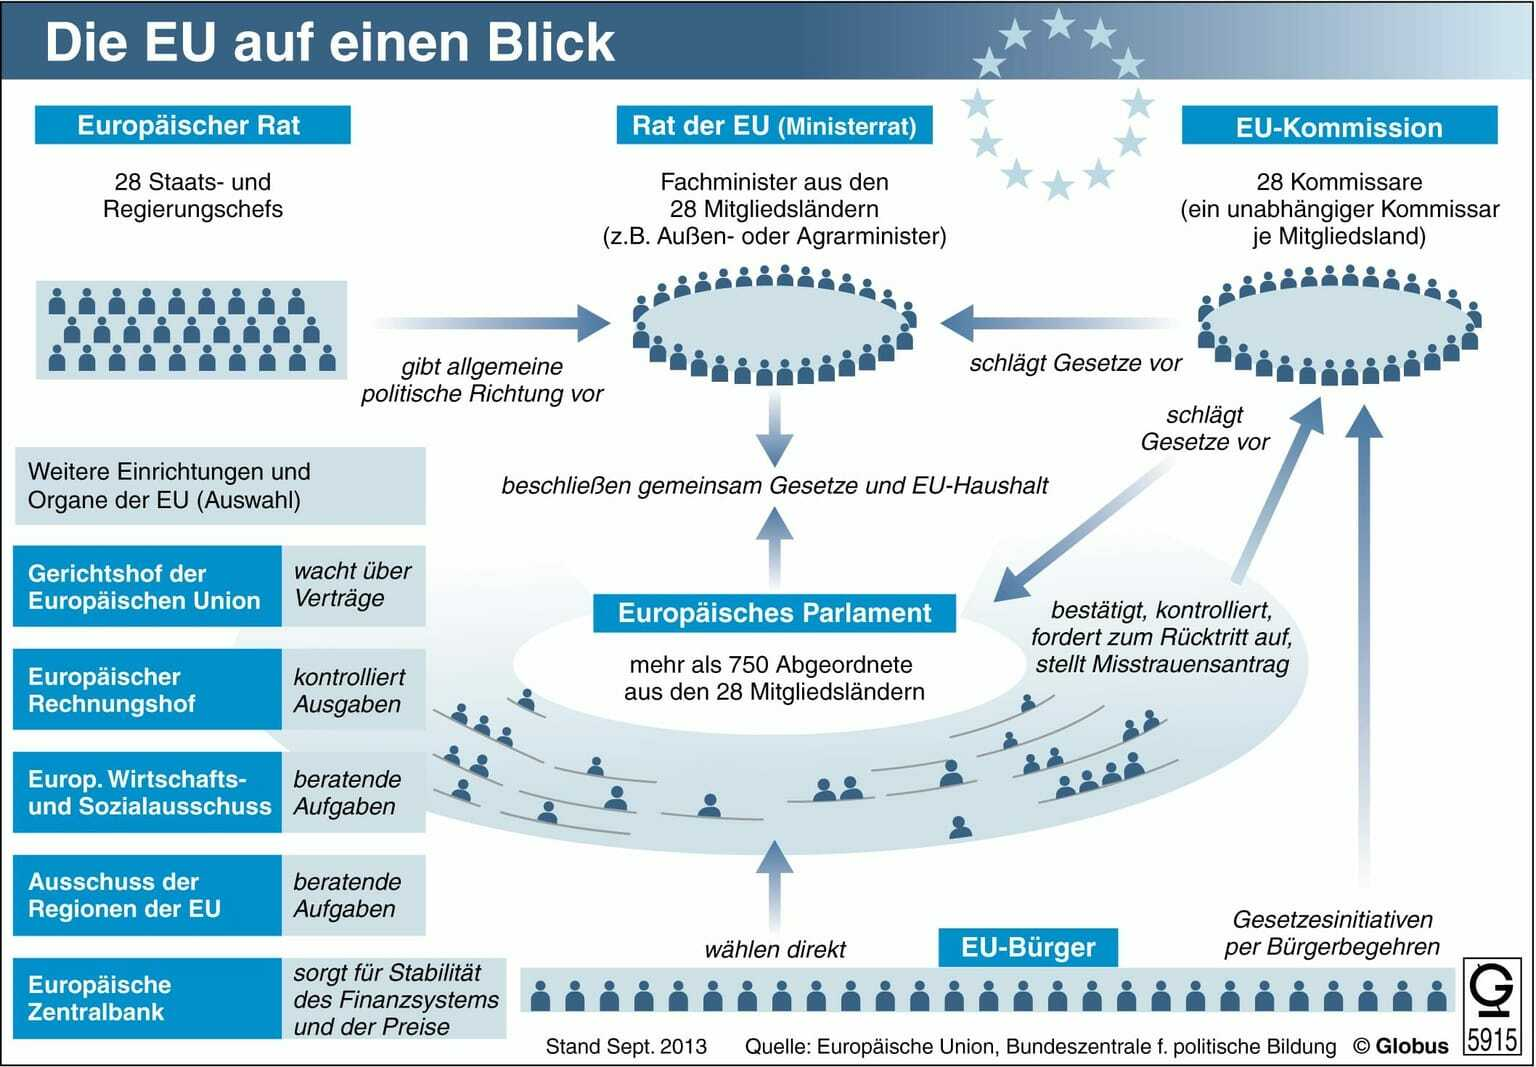
\includegraphics[width=45em]{eu_institutionen.jpg}
  		\caption{Übersicht der EU-Institutionen}
  		\label{fig:eu_institutionen}
	\end{figure}
	
	\subsubsection{Europäischer Rat}
	Der Europäische Rat besteht aus den Staatschefs der jeweiligen Mitgliedsstaaten, einem Präsidenten (momentan Charles Michel), dem Komissionspräsidenten und dem hohen Berater für Außen- und Sicherheitspolitik (die letzteren drei ohne Stimmrecht). Er fällt Grundsatzentscheidungen über die Ausrichtung der EU. Der europäische Rat ist allerding nichts dazu befugt, Gesetze zu erlassen. Der Europäische Rat ist somit eine Art Gipfeltreffen der EU-Staaten, das mindestens viermal im Jahr stattfindet. Insbesondere trifft dieser Rat Entscheidungen bezüglich der EU-Verträge (bspw. Lissabon-Vertrag), die rechtlich gesehen internationale Verträge zwischen einzelnen Staaten sind.

	\paragraph{Rolle}
	Exekutive

	\paragraph{Sitz}
	Brüssel

	\subsubsection{Europäische Kommission}
	Die Europäische Kommission überwacht die EU-Verträge und hat in der Gesetzgebung ein Initiativrecht. Sie besteht aus 26 EU-Komissaren, einem Präsidenten (momentan: Ursula von der Leyen) und einem \textit{hohen Vertreter für die Außen- und Sicherheitspolitik der EU} (momentan: Josep Borrell). Die Komissare werden durch den Präsidenten vorgeschlagen und durch das EP bestätigt. Neben ihrer Rolle in der Gesetzgebung stellt die Komission auch sicher, dass das EU-Recht in den Mitgliedsstaaten eingehalten wird. Außerdem haben EU-Bürger das Recht, die Komission über sogenannte \textit{Europäische Bürgerinitiativen} zur Vorlage von Rechtsvorschriften aufzufordern.

	\paragraph{Rolle}
	Exekutive

	\paragraph{Sitz}
	Brüssel

	\subsubsection{Europäisches Parlament}
	Das Europäische Parlament besteht aus 750 durch die Bürgerinnen und Bürger der EU gewählten Abgeordneten und einem Präsidenten (momentan: Roberta Metsola). Zusammen mit dem Ministerrat beschließt es Gesetze und den EU-Haushalt. Außerdem wählt es den Komissionspräsidenten.

	\begin{wrapfigure}{r}{0.5\textwidth}
		\centering
  		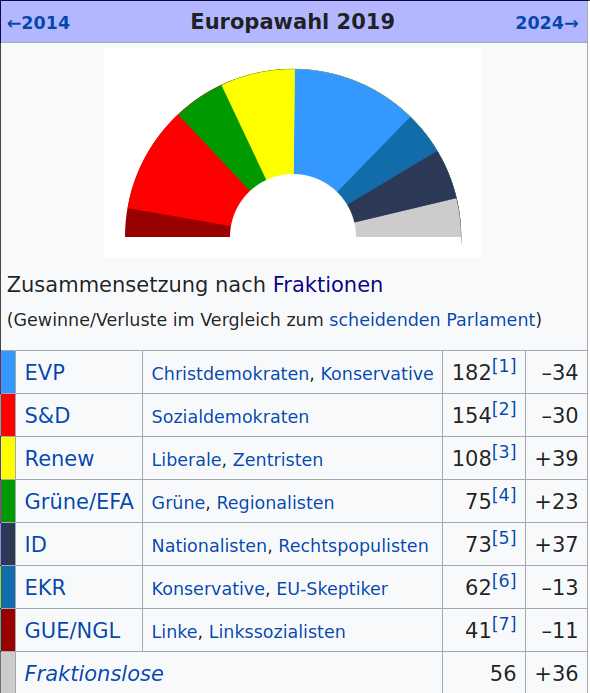
\includegraphics[width=20em]{eu_ep_2019.png}
  		\caption{Sitzverteilung im EP nach 2019}
  		\label{fig:eu_2019}
	\end{wrapfigure}

	\paragraph{Wahl}
	Das EP wird alle fünf Jahre von den EU-Bürgern gewählt. Die 750 Sitze werden dabei nach dem Prinzip der \textit{degressiven Proportionalität} vergeben: Sitze werden zunächst an jedes Land anahnd einer \textit{Mindestvertretung} vergeben, die üblichen Sitze werden dann in immer weniger verhältsnismäßigen Schritten an die bevölkerunsmäßig größten Staaten vergeben. Kleine Länder (bspw. Malta) sind dadurch im Parlament überrepräsentiert, große Länder (bspw. Deutschland) erhalten verhältsnismäßig wenig Sitze. Damit soll sichergestellt werden, dass auch die Interessen kleiner Staaten und insbesondere deren politische Vielfalt angemessen repräsentiert werden, ohne, dass das Parlament zu groß wird. Dadurch repräsentiert ein Sitz aus Malta im Schnitt 14 Millionen Einwohner, während ein deutscher Sitz gerade mal 1 Millionen Einwohner repräsentiert. Das EP ist somit die einzige EU-Institution, die direkt durch die Bürger ggewählt wird.

	\paragraph{Parteien \& Fraktionen}
	Die nationalen Parteien sammeln sich in der Regel in EU-Parteien mit gemeinsamen Interessen. Diese Pareien finden sich dann nochmals zu Fraktionen zusammen, die für gewöhnlich aus einer oder zwei EU-Parteien bestehen (kann aber auch mehr sein). Die sozialdemokratische \textit{Pogressive Allianz der Sozialdemokraten} ist beispielsweise die Fraktion der \textit{Sozialdemokratischen Partei Europas}; an der grünen Fraktion \textit{Die Grünen / Europäische Freie Allianz} sind die \textit{Europäische Grüne Partei}, die \textit{Europäische Freie Allianz} sowie die \textit{Europäische Piratenpartei} und \textit{Volt} beteiligt. 

	\paragraph{Rolle}
	Legislative

	\paragraph{Sitz}
	Straßburg

	\subsubsection{Rat der EU / Ministerrat}
	Der Ministerrat besteht je nach Ressort aus den Ministern der jeweiligen Nationalstaaten. Zusammen mit dem europäischen Parlament beschließt er Gestze und den Haushalt. Der Vorsitz im Rat (Ratspräsidentschaft) wechselt hablbjährlich zwischen den Mitgliedsstaaten (momentan: Schweden), nur beim \textit{Allgemeinen Rat} hat der \textit{Hohe Vertreter für Außen- und Sicherheitspolitik} den Vorsitz.

	\paragraph{Ressorts}
	Beispiele für Konstellationen im Rat der EU sind:
	\begin{itemize}
		\item der \textit{Allgemeine Rat} (Außenminister)
		\item der \textit{Verkehrsrat} (Verkehrsminister)
		\item der \textit{Umweltrat} (Umweltminister)
	\end{itemize}

	Insgesamt gibt es \textit{10} solcher Formationen. 

	\paragraph{Abstimmungen}
	Im Ministerrat wird je nach Frage auf drei verschiedene Arten abgestimmt:

	\subparagraph{Einfache Mehrheit}
	Über Verfahrensfragen wird meist mit einfacher Mehrheit entschieden, die dann vorliegt, wenn die Mehrheit der Mitgliedsstaaten zustimmt.

	 \subparagraph{Qualifizierte Mehrheit}
	 In den meisten Fällen entscheidet der Ministerrat mit der qualifizierten Mehrheit. Diese ist erfüllt, wenn \textit{55\% der Mitgliedsstaaten}, die \textit{65\% der EU-Bevölkerung} repräsentieren, wobei eine \textit{Sperrminorität}, die aus \textit{35\% der Bevölkerung plus ein Mitgliedstaat} besteht (momentan mindestens 4 Staaten), ein \textit{Veto} einlegen können. Für eine qualifizierte Mehrheit müssen momentan mindestens 23 Staaten zustimmen.

	 \subparagraph{Einstimmigkeit}
	 Bei Fragen, die die \textit{Außen- und Sicherheitspolitik} oder die \textit{Steuerpolitik} betreffen, werden Entscheidungen nur einstimmig getroffen.

	\paragraph{Rolle}
	Legislative

	\paragraph{Sitz}
	Brüssel

	\subsubsection{Gerichtshof der EU}
	Als GHdEU wird das gesamte Gerichtssystem der EU bezeichnet. Es besteht jeweils aus

	\begin{enumerate}
		\item dem \textit{Europäischen Gerichtshof}
		\item dem \textit{Gericht der Europäischen Union}
		\item den \textit{Fachgerichten}
	\end{enumerate}

	Der EuGH besteht seit der Montanunion (EGKS) aus einem Richter aus jedem Mitgliedsstaat sowie elf entscheidungsvorbereitenden Generalanwälten. Das EuG  besteht wiederum aus jeweils zwei Richtern pro Mitgliedsstaat, hat allerdings keine Generalanwälte.
	Das bislang einzige Fachgericht war das \textit{Gericht für den öffentlichen Dienst der EU}, welches sich mit dienstrechtlichen Verfahren der Mitarbeiter der EU befasste. Es wurde 2005 aufgebaut und 2016 aufgelöst.

	\paragraph{Rolle}
	Judikative

	\paragraph{Sitz}
	Luxemburg

	\subsubsection{Das wahrgenommene Demokratiedefizit}
	Das Demokratiedefizit in der EU bezieht sich auf Probleme bezüglich der demokratischen Legitimität der EU-Institutionen. Einer der Hauptkritikpunkte ist, dass die Entscheidungen auf EU-Ebene oft von nicht gewählten Beamten oder unabhängigen Expertengremien getroffen werden, anstatt von den direkt gewählten Vertretern der Bürger. Auch ist das Europäische Parlament in vielen Politikbereichen nicht gleichberechtigt mit den anderen EU-Institutionen und hat nicht immer genügend Macht, um seine Rolle als Vertreter der europäischen Bürger vollständig wahrzunehmen. Ein weiterer Kritikpunkt ist, dass die EU oftmals als bürokratisch und undurchsichtig wahrgenommen wird und die Bürgerinnen und Bürger nicht genug Möglichkeiten haben, an Entscheidungen teilzunehmen und ihre Interessen zu vertreten. Außerdem ist eine vollständige Gewaltenteilung nicht immer gegeben: der Ministerrat übernimmt in der EU bspw. die Rolle der Legislative, allerdings besteht er aus Mitgliedern der nationalen Regierungen (Exekutive). So können Regierungen versuchen, Vorhaben, die in ihrem nationalen Parlament keine Mehrheit finden, über die EU durchzusetzen.

	\subsubsection{Gesetzgebungsverfahren in der EU}

	\begin{figure}[!ht]
		\centering
  		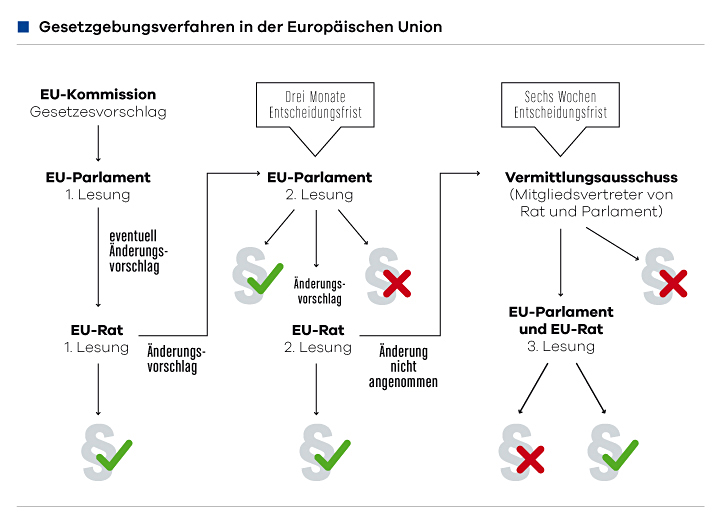
\includegraphics[width=45em]{eu_gesetzverfahren.jpg}
  		\caption{Der Gesetzgebungsprozess in der EU}
  		\label{fig:eu_gesetzverfahren}
	\end{figure}

	Im EU-Recht wird zwischen einer Vielzahl an Rechtsakten unterschieden:

	\paragraph{Verordnung}
	Eine Verordnung ist änhlich einem Gesetz verbindlich und muss von allen EU-Staaten voll umgesetzt werden.

	\subparagraph{Beispiel}
	Die Datenschutz-Grundverordnung regelt den Schutz personenbezogener Daten innerhalb der EU.

	\paragraph{Richtlinie}
	Eine Richtlinie legt ein Ziel fest, das die einzelnen Nationen verwirklichen müssen. Die konkrete Umsetzung ist allerdings den Mitgliedsstaaten überlassen, die jeweils eigene Gesetze erlassen müssen.

	\subparagraph{Beispiel}
	Die Richtlinie 2019/790 regelt das Urheberrecht und die verwandten Schutzrechte im digitalen Binnenmarkt der EU. Auch bekannt als "EU-Urheberrechtsreform".

	\paragraph{Beschluss}
	Beschlüsse, früher auch Entscheidungen, sind verbindliche, unmittelbar geltende Regelungen, die immer nur einen bestimmten Adressatenkreis, etwa ein Land oder ein Unternehmen betreffen.

	\subparagraph{Beispiel}
	Die EU verhängte gegen Microsoft eine Geldstrafe aufgrund von dessen Monopolstellung.

	\paragraph{Empfehlung}
	Die einzelnen EU-Institutionen können unverbindliche Empfehlungen aussprechen.

	\subparagraph{Beispiel}
	Die EU-Komission empfahl in der EU-Luftqualitätsrichtlinie 2008/50/EG  den Mitgliedsstaaten die Verbesserung der Luftqualität in der EU, um die Gesundheit der Bürger zu schützen.

	\paragraph{Stellungnahme}
	Mit Stellungnahmen können sich die wichtigsten EU-Institutionen unverbindlich äußern, ohne irgendwem irgendwelche Verpflichtungen aufzuerlegen

	\subparagraph{Beispiel}
	Die Europäische Kommission gab im Februar 2020 eine Stellungnahme zur nationalen Energie- und Klimaplanung 2021-2030 ab, in der sie die nationalen Energie- und Klimapläne der Mitgliedstaaten bewertete und Empfehlungen zur Umsetzung der EU-Klimaziele bis 2030 gab. Die Stellungnahme soll den Mitgliedstaaten als Orientierungshilfe dienen und zur Verbesserung der nationalen Energie- und Klimapläne beitragen.

	\subsection{Wirtschafts- und Währungsunion EU}
	\subsubsection{Der europäische Binnenmarkt}
	Der europäische Binnenmarkt umfasst ca. 500 Millionen Menschen und hatte 2017 ein BIP von 19.5 Billionen Dollar - mehr als die USA als zweitgrößter Wirtschaftsraum mit 19.4 Billionen Dollar. Innerhalb der EU gibt es eine Zollunion, das heißt, dass es keine innereuropäischen und nur gemeinsame Zölle für Drittstaaten gibt.

	\paragraph{Die vier Grundfreiheiten des europäischen Binnenmarktes}
	\begin{itemize}
		\item Freiheit der Waren: ungehinderter Import und Export
		\item Freiheit der Dienstleistungen: Niderlassungsfreiheit
		\item Freiheit für Arbeitskräfte: jeder kann arbeiten, wo er will
		\item Freiheit des Kapitals: Investieren und Geld anlegen, wo man will
	\end{itemize}

	\subsubsection{Schengen-Raum}
	Das Schengener Abkommen sieht vor, dass es keine innereuropäischen Personenkontrollen mehr geben soll. Die außereuropäischen Grenzen sollen dafür besonders geschützt werden. Teilnehmer sind alle EU-Staaten mit der Ausnahme von Rumänien und Bulgarien (aufgrund von strukturellen Mängeln bei der Grenzsicherung), Irland (aufgrund der komplizierten Situation mit Nordirland und Großbrittanien) und Zypern (aufgrund der Problematik mit Nord-Zypern). Neben den EU-Staaten nehmen noch die Schweiz, Liechtenstein, Norwegen und Island am Schengen-Raum teil.

	\subsubsection{Die Eurozohne}
	Der Euro ist die gemeinsame Währung der EU. In einer Währungsunion geben die einzelnen Mitglieder ihre individuellen Währungspolitiken auf und geben die geldpolitischen Kompetenzen an eine gemeinsame Behörde ab; im Fall des Euros ist dies die Europäische Zentralbank in Frankfurt am Main. Eine einheitliche Währung stärkt einen gemeinsamen Binnenmarkt und macht schwankende Wechselkurse und Transaktionskosten überflüssig. Der Euro ist momentan wertvoller als der amerikanische Dollar, was für seine Stabilität spricht. Wichtig für eine Währungsunion ist eine möglich einheitliche Wirtschafts- und Finanzpolitik, die vor Staatsüberschuldung schützen und die Währung somit Krisenfest machten

	\paragraph{Teilnehmer}
	Am Euro nehmen alle EU-Staaten mit Ausnahme von Schweden, Dänemark, Polen, Tschechien, Ungarn, Rumänien und Bulgarien teil. Die Kleinststaaten Andorra, Monaco, San Marino und der Vatikan haben ebenfalls eigene Euromünzen. Der Kosovo und Montenegro benutzen den Euro ebenfalls, allerdings ohne Erlaubnis der EU - daher haben sie auch keine eigenen Münzen.

	\subsubsection{EU-Haushalt}
	Die EU kann keine eigenen Steuern erheben, weshalb sie sich ihren Haushalt über sogenannte "Eigenmitte  finanzieren muss:

 	\begin{itemize}
		\item 13\% Traditionelle Eigenmittel (z.B. Zölle)
		\item 11\% Mehrwertsteuer-Eigenmittel (0,3\% Anteil an der Mehrwertsteuer der EU-Staaten; in Deutschland nur 0,15\%)
		\item 75\% BNE-Eigenmittel (Beiträge der EU-Mitglieder prozentual am BNE)
		\item 1\% Sonstige Einnahmen (z.B. Zinsen)
	\end{itemize}

	\paragraph{Nettozahler- und Empfänger}
	Aus der Differenz zwischen den in die EU eingebrachten Leistungen und den von der EU erhaltenen Leistungen ergibt sich, ob ein Staat mehr Geld zahlt (Nettozahler) oder mehr bekommt (Nettoempfänger). Auch, wenn Deutschland mehr Geld an die EU zahlt, als es bekommt, profitiert Deutschland von der EU; insbesondere über die Zollfreiheit, die politische Stabilität, den freien Personenverkehr und andere Aspekte.

	\subsection{Europäische Integrationsmodelle}
	\subsubsection{Modelle}
	Für die Zukunft der EU gibt es 5 Modellvorschläge aus unterschiedlichen Richtungen:

	\paragraph{Europäischer Bundesstaat}
	Der Europäische Bundesstaat zeichnet sich ähnlich dem deutschen Föderalismus durch eine klare Kompetenzabgranzung zwischen der EU und den Mitgliedstaaten aus. Jede Ebene hat hierbei demokratisch legitimierte Regierungen: auch auf der EU-Ebene soll eine Regierung gewählt werden, etwa durch eine Wahl eines Regierungschefs durch das Parlament. Der Bundesstaat würde außerdem über eine Verfassung inklusive einer Erklärung der Grundrechte sowie ein Steuersystem verfügen. Die Zuständigkeiten etwa in Bereichen der Außen-, Sicherheits-, Wirtschafts- und Währungspolitik müssten klar definiert sein. Befürworter sind insbesondere die 6 Gründungsmitglieder.

	\paragraph{Europäischer Staatenbund}
	Im Europäischen Staatenbund würden die souveränen Staaten zwar weiter zusammenarbeiten, allerdings würde keine Regierung ihr Entscheidungsrecht abgeben. Entscheidungen auf europäischer Ebene würden immer einstimmig getroffen werden. Ein Parlament ist entweder nicht notwendig oder spielt eine untergeordnete Rolle, um die Handlungsmöglichkeiten der Regierungen nicht zu beschränken. Nachteile dieses Modells wären langwierige Entscheidungen, nicht zufriedenstellende Kompromisse und eine geringere Legitimierung von Entscheidungen auf europäischer Ebene. Auch gestalten sich Überprüfungen durch unabhängige Gerichte schwierig. Befürworter dieses Systems sind insbesondere Großbritannien und die skandinavischen Länder, aber auch Osteuropäische Stimmen.

	\paragraph{Europa der Regionen}
	In einem Europa der Regionen bekommen einzelne Regionen, die überschaubare politische Einheiten darstellen, mit denen  ihre Bewohner sich häufig identifizieren können, mehr Macht auf europäischer Ebene. Die Problemnähe der Regionen würde eine höhere Legitimation von Entscheidungen und einen effizienteren Entscheidungsfindungsprozess bedeuten. Diese Regionalisierung würde auch ein Gegengewicht zu der Zentralisierung der EU-Institutionen darstellen. Allerdings ist nicht klar, wie die Zusammenarbeit der Regionen auf europäischer Ebene genau aussehen soll. Ein Modell hierfür ist ein beratender "Ausschuss der Nationen". 

	\paragraph{Differenzierte Integration}
	Das Modelll der differenzierten Integration setzt voraus, dass es schwierig ist, Einigungsfortschritte zu erzielen, wenn die Mitgliedstaaten unterschiedliche Vorraussetzungen haben. Daher sollen neue Zusammenarbeitsformen erschlossen werden, in denen die Mitgliedstaaten in unterschiedlichen Zusammensetzungen an unterschiedlichen Aufgaben arbeiten. Dieses Modell hat nochmals im wesentlichen drei Varianten:

	\subparagraph{Europa der zwei Geschwindigkeiten}
	In diesem Modell werden zwar gemeinsame Ziele definiert, allerdings sind die Zeiträume, in denen die Mitgliedstaaten diese Ziele erfüllen müssen, unterschiedlich.

	\subparagraph{Staatliche Sonderwege}
	Einzelne Staaten können sich dazu entscheiden, an bestimmten Entwicklungen gar nicht oder erst später teilzunehmen. Das kann zwar Blockaden lösen, führt potentiell aber auch zu werniger Solidarität zwischen den Staaten.

	\subparagraph{Varibale Geometrie}
	Die einzelnen Mitgliedstaaten finden sich in kleineren Gruppen zusammen, um an einzelnen Verfahren bzw. Entwicklungen teilzunehmen.

	\paragraph{Festung Europa}
	Das Gegenbild der "Festung Europa" beschreibt ein Szenario, in dem die Menschen innerhalb der Grenzen Europas in Zufriedenheit und Sicherheit leben, während außerhalb der Grenzen Armut und ein "Kampf ums Überleben" gegeben sind. Europa schottet sich demnach durch eine Beschränkung der Migration von der Außenwelt ab. Dieses Szenario wird als unerwünscht und unrealistisch betrachtet, da Migration nicht wirklich aufhaltbar sei und der demographische Wandel einen Zuzug von neuen Erwerbstätigen notwendig macht. Europa solle besser eine gute Nachbarschaft zu den außereuropäischen Staaten pflegen und Notwendigkeiten, das eigene Land zu verlassen, abbauen.

	\subsubsection{Integrationstheorien}
	\paragraph{Föderalismus / Supranationalität}
	Die einzelnen Staaten blieben zwar im Grunde bestehen, teilen sich ihre Kompetenzen aber mit einem übergeordneten Gesamtsystem. Es gibt also keinen europäischen "Superstaat", sondern eine parallele Existenz von supranationalen und nationalen Institutionen. Das entsprechende Modell wäre das des europäischen Bundesstaates

	\paragraph{Intergouvernementalismus}
	Die Nationalstaaten bleiben bestehen und treffen nur gemeinsame Absprachen, ohne, dass es supranationale Institutionen mit mehr Entscheidungsgewalt gibt. Instrumente sind etwa Geipfeltreffen oder Regierungskonferenzen. Ziel ist der nationale Machterhalt, Faktoren sind das Nationalbewusstsein, der Nationalismus als Ideologie und andere nationale Interessen. Ein Modell wäre hier der Europäische Staatenbund. 

	\paragraph{(Neo-) Funktionalismus}
	Der Neofunktionalismus besagt, dass die Integration durch die Schaffung funktionaler Zusammenarbeit in begrenzten Politik- oder wirtschaftsbereichen vorangetrieben wird, was zu einer stärkeren Integration in anderen Bereichen führt. Dieser Prozess wird als "Spillover" bezeichnet und kann politische Integration auf supranationaler Ebene auslösen. Die Theorie betont auch die Bedeutung von wirtschaftlicher Interdependenz und Vertrauen zwischen den Mitgliedsstaaten, um die Integration voranzutreiben. Kritiker argumentieren jedoch, dass der Neofunktionalismus die politischen Realitäten und Interessen der Mitgliedsstaaten vernachlässigt und die Integration auf Kosten der nationalen Souveränität vorantreibt.

\end{document}
